\documentclass[10pt,twocolumn]{article}
\usepackage[T1]{fontenc}
\usepackage{newtxtext,newtxmath}
\usepackage[a4paper,margin=17mm,columnsep=6mm]{geometry}
\usepackage{graphicx,booktabs,amsmath,xcolor,microtype,url,tabularx,multirow}
\usepackage[font=small,labelfont=bf,skip=4pt]{caption}
\usepackage{subcaption}
\usepackage[numbers,sort&compress]{natbib}
\usepackage{tikz}
\usetikzlibrary{arrows.meta,positioning,fit,calc}
\usepackage[hidelinks]{hyperref}
\usepackage{siunitx}
\usepackage{placeins}
\renewcommand{\topfraction}{0.9}\renewcommand{\bottomfraction}{0.8}\renewcommand{\textfraction}{0.07}
\renewcommand{\floatpagefraction}{0.75}\renewcommand{\dbltopfraction}{0.9}\renewcommand{\dblfloatpagefraction}{0.75}
\setcounter{topnumber}{3}\setcounter{dbltopnumber}{3}\setcounter{totalnumber}{6}
\sisetup{detect-all,group-minimum-digits=4}
\graphicspath{{figures/}}
\setlength{\tabcolsep}{4pt}
\renewcommand{\arraystretch}{1.08}
\newcommand{\metre}{\,m}
\makeatletter\newcommand{\tabinput}[1]{\@@input #1 }\makeatother

\title{\vspace{-6mm}\Large\bfseries Georeferencing a 1926 Survey of India Sheet:\\ Learned Matching, Classical Matching and Manual Control Points\\ Compared on Held-Out Ground Truth}
\author{Saksham Sharma\\[2pt]
\normalsize Code, data provenance and all outputs: \url{https://github.com/1sakshm/MapAlign}\\
\normalsize Interactive version: \url{https://mysore-1926.pages.dev}}
\date{October 2026}

\begin{document}
\maketitle

\begin{abstract}
\noindent
Large archives of colonial Survey of India topographic sheets are now openly available as scans, but almost none of them are georeferenced. We measure how well three standard approaches place one such sheet, 57\,D/11 \emph{Mysore} (1:63,360, published 1926), on modern ground. The three are a pretrained LoFTR matcher with MAGSAC++, SIFT with MAGSAC++, and a least-squares homography fitted to manually selected control points. The modern reference is OpenStreetMap (OSM), rendered by us to a 5\,m grid in WGS\,84/UTM~43N. All methods share one coordinate chain and one evaluation, scored in metres at 12 held-out points whose truth comes from OSM vector geometry.

SIFT produced no valid transform. Even on tiles that had already been aligned, only 4.75\% of its matches were correct, against a chance rate of 4.31\%. LoFTR gave 389 RANSAC inliers out of 601 matches and reached a held-out median error of 53.9\metre{} (RMSE 77.4\metre). The 7-point manual fit reached 73.9\metre{} (RMSE 102.4\metre). LoFTR was closer at 9 of 12 points (exact Wilcoxon $p=0.043$), but the bootstrap interval for the median paired difference, $[-44.0, +2.5]$\metre, includes zero, and no secondary test against this manual fit survives a multiple-testing correction. LoFTR does clearly beat georeferencing from the four printed sheet corners alone (median 169.8\metre, Holm-adjusted $p=0.012$). A blind, timed human re-pick of the control points made the manual fit worse (median 123.7\metre), and LoFTR was then closer at all 12 points. Of two sparse learned matchers added afterwards, DISK with LightGlue failed like SIFT, while ALIKED with LightGlue reached a 54.6\metre{} median but a higher RMSE (104.9\metre). A known-transform benchmark puts LoFTR's own error at 2--4\metre, so nearly all of the remaining error comes from the map, a century of change and the reference, not from the matcher.

An affine model did as well as the homography, and polynomial and thin-plate-spline models did no better. Both methods carry a measurable mean bias of 33--56\metre. The sheet's printed graticule is offset from WGS\,84 by roughly 100\metre, consistent with a Kalianpur datum. We release the pipeline and the exact inputs. A re-run reproduces every number in this paper bit for bit on the original machine, and to 0.01\metre{} on Linux.
\end{abstract}

\section{Introduction}

Between the 1860s and the 1960s the Survey of India mapped most of South Asia at one inch to the mile. These sheets record settlements, canals, tanks and railways that have since been rebuilt or erased. They are some of the best evidence of how the region's land use changed over the twentieth century. Thousands of them are now freely available as scans~\citep{brown_soi_zenodo}. Using a scan alongside modern data needs one step first: georeferencing, the estimation of a mapping from scan pixels to geographic coordinates.

The usual way to do this is to place ground-control points (GCPs) by hand, at features that can be found on both the old sheet and a modern reference. That works, but it is slow, it depends on the operator, and after a century of change the features that survive are scarce and unevenly spread. Automatic feature matching is the obvious alternative. Detector-based pipelines built on SIFT~\citep{lowe2004sift} have long been used in map processing~\citep{chiang2014survey}. More recently, detector-free matchers such as LoFTR~\citep{sun2021loftr} have shown that dense transformer features can match low-texture image pairs where keypoints fail.

A 1926 lithograph and a modern vector rendering are a hard pair for either kind of matcher. The two images share no photometric appearance. Symbols, lettering, line weights and colours all differ, and part of the content itself has changed. Whether matchers transfer to this setting is an empirical question. Answering it fairly needs a protocol in which the methods use the same coordinate chain and are scored in metres on points they never saw.

This paper reports such a comparison on a single sheet. Our contributions are modest and practical:
(i)~a fully reproducible pipeline that takes a Zenodo scan and an OSM extract to georeferenced GeoTIFFs, with explicit pixel conventions and an exact (non-affine) resampling of the projective transform;
(ii)~a held-out evaluation in metres, with a written point-selection protocol, quality control that never looks at method output, and a hash lock on the test set;
(iii)~a diagnosis of \emph{why} SIFT fails on this pair, separate from \emph{whether} it fails;
(iv)~an analysis of the residual errors, including bias, an affine-versus-projective comparison and the datum of the printed graticule.
We make no claim of methodological novelty, and a single sheet does not support general claims about historical maps.

\section{Related work}
\label{sec:related}
Automatic georeferencing of historical maps is usually framed as registration between an old map and a reference that is already georeferenced. \citet{chiang2014survey} survey the earlier, mostly rule-based work on extracting and aligning map content. Recent pipelines rely on learned local features. \citet{vaienti2025georef} transfer georeferencing from already georeferenced maps of Jerusalem to new ones with SuperPoint and SuperGlue~\citep{detone2018superpoint,sarlin2020superglue}, removing outliers with RANSAC and a Delaunay-consistency test. They report an RMSE below 1\% of the map diagonal for 71 of 86 maps, and find that about 100 matched keypoints separate reliable from unreliable results. JADIS SuperMapRealigner~\citep{petitpierre2026realigner} segments the road network first and then matches keypoints with the same SuperPoint--SuperGlue pair; it was developed on maps of Paris. \citet{wu2026urbanchange} align historical maps of Paris (1868--1937) as the first stage of a framework that measures urban change.

Our setting differs from these in three ways. The reference is a modern vector database (OSM) rendered in a style unlike any historical map, so the pair is cross-era as well as cross-style. The sheet is a rural and small-town Survey of India sheet rather than a city plan. And the comparison is scored at held-out control points, in metres, with a locked test set and the same estimator for every method. We also test a detector-free matcher (LoFTR~\citep{sun2021loftr}) against classical and sparse learned ones (DISK and ALIKED with LightGlue~\citep{tyszkiewicz2020disk,zhao2023aliked,lindenberger2023lightglue}).

Map content recognition is the other half of making such archives usable. Work on segmenting heterogeneous map collections~\citep{petitpierre2026semap}, on studying cartography across hundreds of thousands of catalogued maps~\citep{petitpierre2025thesis}, and on detecting, recognising and linking map text~\citep{lin2025maptext} points the same way: models that generalise across collections rather than one series. Survey of India sheets are a large, little-studied series for such work, and an accurate georeference is a precondition for comparing their content with today's.

\section{Data}

\begin{figure}[t]
\centering
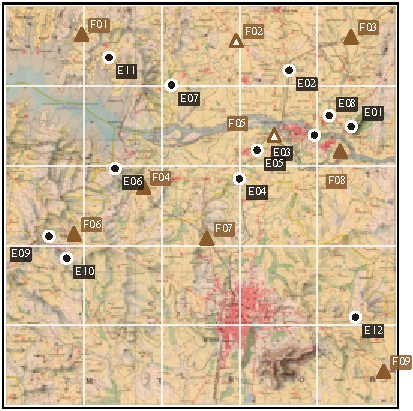
\includegraphics[width=\columnwidth]{fig1_sheet_gcps}
\caption{Sheet 57\,D/11 (1926), cropped to the neatline, with the $5\times5$ design grid used for point selection. Brown triangles are fitting points for the manual baseline; the hollow ones (F02, F05) were removed by quality control before fitting. Black circles are the 12 held-out evaluation points. No evaluation point falls in the southern row or in Mysore city (bottom centre), where 1926 features could not be matched with confidence.}
\label{fig:sheet}
\end{figure}

\paragraph{Historical sheet.}
We use Survey of India sheet No.~57\,D/11, \emph{Mysore}, Mysore District, at 1:63,360. It was surveyed in season 1924--25 and published in 1926 under Col.~C.\,P.~Gunter, Officiating Surveyor General. The scan comes from the Old Survey of India Maps collection on Zenodo~\citep{brown_soi_zenodo} (record 8388121, CC\,BY\,4.0). It is a $5898\times6828$ pixel JPEG at 300\,dpi, which corresponds to a nominal 5.36\metre{} per pixel on the ground. The sheet carries a University of Michigan library stamp. Its neatline spans $76^\circ30'$--$76^\circ45'$\,E and $12^\circ15'$--$12^\circ30'$\,N, about $27.2\times27.6$\,km. The graticule is ticked every $5'$, with no projected grid.

We chose this sheet over two other Karnataka candidates (57\,H/9 of 1927 and 57\,D/11 of 1947) for three reasons. Its scan is clean and flat. Its northern half, along the Cauvery around Srirangapatna, has many features that survive. And it contains three railway lines. The Krishnarajasagara dam in its north-west corner was still under construction in 1926, so that corner has changed beyond use (Fig.~\ref{fig:sheet}). We verified the MD5 checksum published by Zenodo and recorded the SHA-256 of the exact file used.

\paragraph{Modern reference.}
We downloaded OSM features~\citep{osm} with a single Overpass query covering the sheet plus a $0.03^\circ$ margin. The query returned 32{,}355 ways, 283 nodes and 10 relations (snapshot 2026-10-18 18:43\,UTC): roads, railways, waterways, water bodies and places. We render these ourselves into a $6785\times6900$ GeoTIFF in WGS\,84/UTM zone~43N (EPSG:32643) at 5\metre{} per pixel, with an exact north-up affine geotransform. The style loosely follows the 1926 palette: red roads, black railways, blue water. Rendering it ourselves, instead of using web tiles, fixes the pixel-to-metre mapping exactly and respects the OSM tile policy.

\paragraph{Coordinate reference.}
All positional errors are computed in EPSG:32643. At the sheet centre, UTM distance differs from geodesic distance by 0.08\metre{} over 10\,km~\citep{snyder1987projections}, which is negligible here. The printed graticule is on a pre-WGS\,84 Indian (Kalianpur) datum that we did not identify. PROJ has no real Kalianpur~1880$\to$WGS\,84 transformation. We therefore never use printed coordinates as truth, and in Section~\ref{sec:datum} we measure their offset instead.

\section{Methods}

\begin{figure*}[t]
\centering
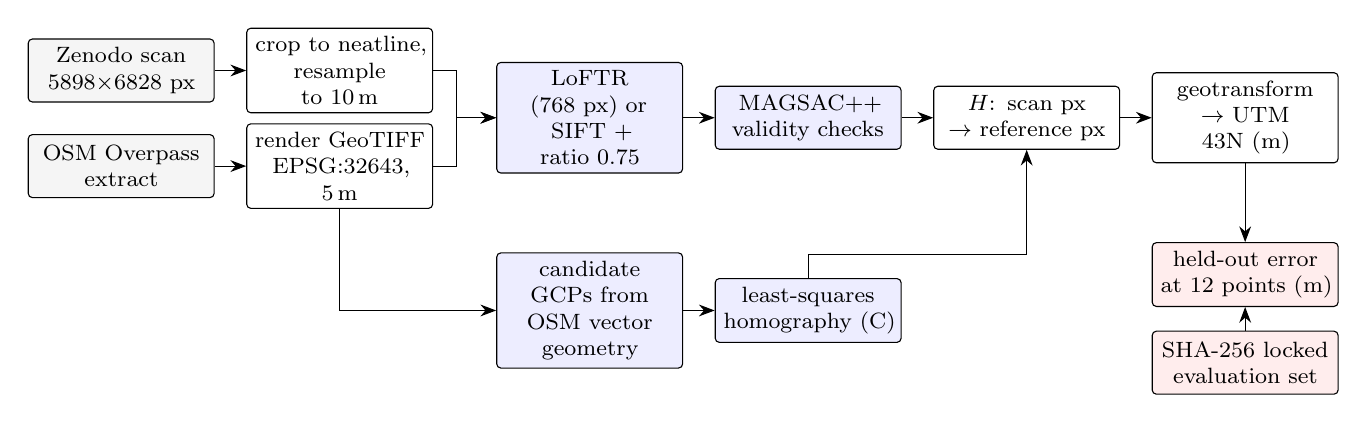
\begin{tikzpicture}[
  node distance=4mm and 4mm,
  box/.style={draw, rounded corners=1.5pt, align=center, font=\footnotesize, inner sep=3pt, minimum height=8mm, text width=21.5mm},
  data/.style={box, fill=black!4},
  meth/.style={box, fill=blue!7},
  ev/.style={box, fill=red!7},
  >={Stealth[length=2mm]}]
\node[data] (scan) {Zenodo scan\\5898$\times$6828 px};
\node[box, right=of scan] (prep) {crop to neatline,\\resample to 10\,m};
\node[data, below=of scan] (osm) {OSM Overpass\\extract};
\node[box, right=of osm] (render) {render GeoTIFF\\EPSG:32643, 5\,m};
\node[meth, right=8mm of prep, yshift=-6mm] (match) {LoFTR (768 px) or\\SIFT + ratio 0.75};
\node[meth, right=of match] (ransac) {MAGSAC++\\validity checks};
\node[box, right=of ransac] (H) {$H$: scan px\\$\to$ reference px};
\node[box, right=of H] (geo) {geotransform\\$\to$ UTM 43N (m)};
\node[meth, below=of match, yshift=-6mm] (gcp) {candidate GCPs from\\OSM vector geometry};
\node[meth, right=of gcp] (ls) {least-squares\\homography (C)};
\node[ev, below=of geo, yshift=-6mm] (eval) {held-out error\\at 12 points (m)};
\node[ev, below=3mm of eval] (lock) {SHA-256 locked\\evaluation set};
\draw[->] (scan) -- (prep); \draw[->] (osm) -- (render);
\draw[->] (prep.east) -- ++(3mm,0) |- (match.west); \draw[->] (render.east) -- ++(3mm,0) |- (match.west);
\draw[->] (match) -- (ransac); \draw[->] (ransac) -- (H); \draw[->] (H) -- (geo);
\draw[->] (render.south) |- (gcp.west); \draw[->] (gcp) -- (ls); \draw[->] (ls.north) -- ++(0,3mm) -| (H.south);
\draw[->] (geo) -- (eval); \draw[->] (lock) -- (eval);
\end{tikzpicture}
\caption{Pipeline. All three methods produce the same object, a $3\times3$ homography from full-resolution scan pixels to reference pixels, and are scored by one evaluation. Blue: method-specific steps. Red: evaluation, which no method can see.}
\label{fig:pipeline}
\end{figure*}

\subsection{Coordinate chain and conventions}
Every method estimates a matrix $H$ that maps a scan pixel $\mathbf{x}$ (OpenCV pixel-centre convention, full resolution) to a reference pixel. The reference geotransform $A$ then maps that pixel to EPSG:32643:
\begin{equation}
\hat{\mathbf{p}} = A\,\pi(H\tilde{\mathbf{x}}),\qquad \pi([u,v,w]^\top)=[u/w,\,v/w]^\top,
\end{equation}
where $\tilde{\mathbf{x}}$ is homogeneous. Rasterio's geotransform addresses pixel corners, so $A$ includes a half-pixel shift. Matches found at working resolution are mapped back to full resolution through explicit crop-and-resize matrices. We unit-test these against \texttt{cv2.resize} to $0.05$ pixel. Figure~\ref{fig:pipeline} summarises the chain.

\subsection{Preprocessing}
We crop the scan to its neatline. The four corners were placed by eye and then refined to the darkest line pixel, giving a $5048\times5170$ pixel crop. We resample both images to a common nominal 10\metre{} per pixel ($2708\times2773$ and $3392\times3450$ pixels) and convert them to greyscale.

\subsection{Method A: LoFTR}
We use Kornia's~\citep{riba2020kornia} implementation of LoFTR with the \emph{outdoor} weights~\citep{sun2021loftr}, in evaluation mode without gradients. LoFTR's coarse stage compares every $1/8$-resolution cell of one image with every cell of the other. At 10\metre{} per pixel the full sheet would need a similarity matrix of about $10^{10}$ entries, so we scale both images by one common factor until the longer side is at most 768 pixels. That gives inputs of $600\times616$ and $752\times768$ pixels at about 44.9\metre{} per pixel, with ground resolution kept equal across the pair. All 601 matches are kept regardless of confidence (mean confidence 0.52) and passed to the robust estimator.

\subsection{Method B: SIFT}
We run OpenCV SIFT~\citep{lowe2004sift} with default parameters on the 10\metre{} images. Descriptors are matched by brute-force $L_2$ two-nearest-neighbour search, and the ratio test is applied at 0.75.

\subsection{Shared robust estimation}
Both automatic methods use OpenCV's USAC implementation of MAGSAC++~\citep{barath2020magsacpp}, a descendant of RANSAC~\citep{fischler1981ransac}. Our configuration sets a random seed of 42, but OpenCV's flag-based USAC call ignores it and uses a fixed internal random state (0). The results are therefore deterministic, and Section~\ref{sec:robust} reports how much they vary over 200 explicit seeds. The inlier threshold is 3 pixels at the resolution where the matcher located its points. That is 30\metre{} for SIFT and 13.5 working pixels, about 135\metre, for LoFTR. We allow $1.2\times10^6$ iterations, the standard sample count $N=\log(1-p)/\log(1-w^4)$ for confidence $p=0.999$ at an inlier ratio as low as $w=0.05$.

A model is rejected if it fails any of these checks: finite entries; condition number $<10^7$; positive determinant; ratio of singular values $<10$; image corners on the same side of the horizon line; a convex mapped outline; mapped corners within half an image of the reference. A rejected model is recorded as a failure, and it is never repaired.

\subsection{Method C: manual control points}
We computed 1{,}053 candidate GCPs from OSM vector geometry: exact railway--road, railway--water and road--water intersections, junctions of major roads, stations and landmark centroids. A candidate's EPSG:32643 coordinates are its truth. For each candidate we located the corresponding pixel on the 1926 scan in zoomed crops with a 10 pixel grid. The crops were centred using only the four printed sheet corners, so no method's transform could steer the picking. Candidate locations were first proposed with the help of a large language model assistant working from these crops. The author then checked all 21 resulting points, fitting and evaluation, against the scan and the OSM render, and accepted all of them.

A feature was accepted only if it exists in 1926 with the same geometry and can be located to about $\pm5$ pixels ($\pm27$\metre). The fit is an ordinary least-squares homography on the accepted fitting points (Hartley and Zisserman~\citep{hartley2004mvg}, DLT without RANSAC). That is the same model family as Methods A and B.

\subsection{Evaluation protocol}
\paragraph{Freezing.} All parameters were frozen on 19 October 2026, before any evaluation point existed. Three settings were changed during development, and each change was justified on development data only. (i)~The LoFTR input size went from 1280 to 768 pixels, chosen by a rule fixed before the sweep: the most matches within 1\,km of the position predicted by the printed corners (Table~\ref{tab:sweep}). (ii)~The iteration count went from $10^4$ to $1.2\times10^6$. (iii)~The threshold changed from a fixed 3 working pixels to the matcher-relative rule above. SIFT was given the same estimator settings, and eight preprocessing variants, for parity.

\paragraph{Point selection and quality control.}\label{sec:gcp}
The written protocol divides the neatline into a $5\times5$ grid. It asks for one fitting point in each of 13 cells and 20 evaluation points spread over the sheet, each at least 1\,km from every fitting point. We screened every point with a test that uses no method output. For each point we take the offset between its picked pixel and the pixel predicted by the printed corners, and flag the point if that offset lies more than 3 robust standard deviations ($1.4826\times$MAD) from the median.
\begin{itemize}
\item On the fitting set the test removed F02, an apparently realigned road with $z_E=-7.4$, and F05 ($z_E=3.6$). That left 7 fitting points.
\item On the evaluation set it flagged two picking errors: a wrong road (E12) and a position that had been extrapolated instead of read (E06). Both were re-examined and corrected. None was dropped, and after correction the largest $|z|$ is 2.99.
\end{itemize}

\paragraph{Shortfall.} Only 12 evaluation points could be established instead of 20. Most candidates failed for one of three reasons: the feature postdates 1926 (the Varuna canal network, ring roads); the feature has moved (inside Mysore city the Nanjangud railway lies about 280\metre{} from its 1926 course, consistent with gauge conversion); or the junction is ambiguous. The evaluation file was locked by SHA-256 before any prediction was computed, and the evaluation code refuses to run if it changes.

\paragraph{Metrics.} For point $i$ the error is
\begin{equation}
e_i=\sqrt{(E_i-\hat E_i)^2+(N_i-\hat N_i)^2}\quad\text{(m, EPSG:32643)}.
\end{equation}
We report the mean, median, RMSE, population standard deviation, 90th percentile, minimum and maximum. Methods are compared on the same points, paired: an exact two-sided Wilcoxon signed-rank test~\citep{wilcoxon1945} and a percentile bootstrap 95\% interval for the median paired difference, with 20{,}000 resamples~\citep{efron1993bootstrap}. With $n=12$ both are low-powered, and we read them as descriptive.

\section{Results}

\begin{table*}[t]
\centering
\caption{Held-out positional error in metres (EPSG:32643), homography model, the same 12 points for every method. Runtimes are wall-clock on a Ryzen~7 5800HS CPU.}
\label{tab:results}
\begin{tabular}{lrrrrrrrr}
\toprule
Method & $n$ & Median & Mean & RMSE & Std & P90 & Min & Max \\
\midrule
\tabinput{tables/results.tex}
\bottomrule
\end{tabular}
\vspace{2pt}

\small
\begin{tabular}{lcccc}
Method & Matches & Inliers & Inlier ratio & Runtime (s) \\
\midrule
LoFTR + MAGSAC & 601 & 389 & 64.7\% & 18.3 \\
SIFT + MAGSAC & 594 & 26 (degenerate) & 4.4\% & 14.6 \\
Manual GCPs & 7 points & -- & -- & 0.15 (fit only) \\
\end{tabular}
\end{table*}

\subsection{SIFT does not transfer to this map pair}
SIFT found 79{,}923 keypoints on the scan and 18{,}547 on the render. Only 594 matches passed the ratio test, and just 2 of them landed within 1\,km of where the printed corners place them. MAGSAC++ found a 26-inlier model, but it was singular: condition number $8.4\times10^{13}$, a zero singular value, and corners mapped past the horizon line. The validity checks therefore rejected it (Fig.~\ref{fig:corr}b).

None of the eight preprocessing variants helped (Table~\ref{tab:siftvar}), including colour-layer separation of roads, water and linework, and ground resolutions from 10 to 45\metre. Colour layers raised the number of ratio-test matches to 1{,}351, but at most 5 of them were near the prior.

To separate ``SIFT cannot match these images'' from ``RANSAC could not find the model'', we warped the scan with the printed-corner prior and matched 25 aligned tiles of $512\times512$ pixels (5.1\,km). A match counts as correct if it lands within 600\metre{} of its own position. Matches placed at random would be correct 4.31\% of the time. SIFT reached 4.75\% (97 of 2{,}041) and LoFTR 12.92\% (321 of 2{,}485) (Fig.~\ref{fig:diag}a). SIFT's descriptors therefore carry essentially no information about this pair, even when the geometry is handed to it.

\begin{figure*}[t]
\centering
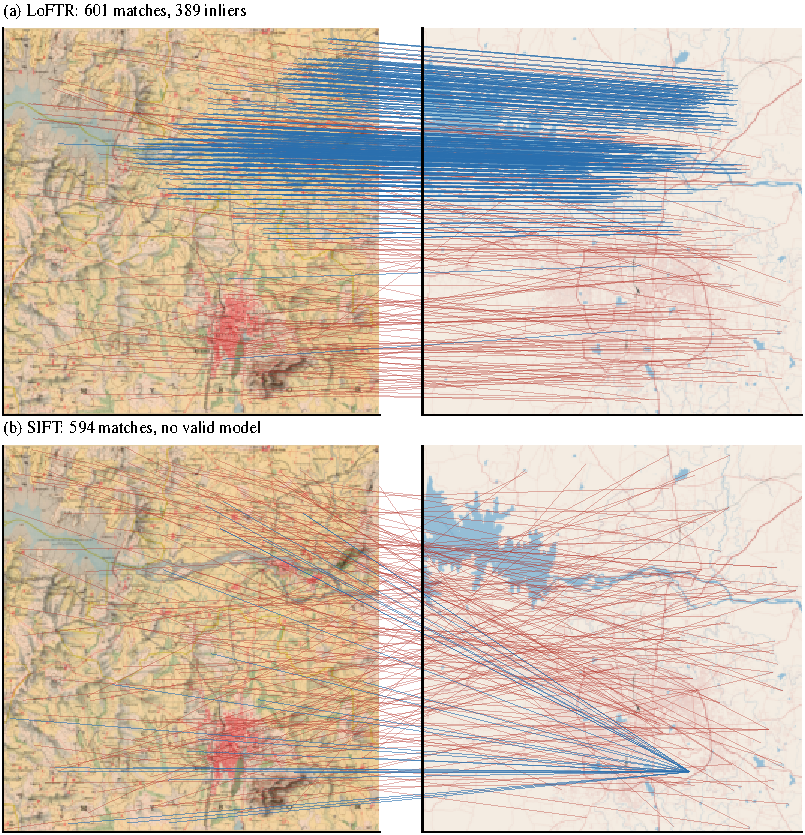
\includegraphics[width=\textwidth]{fig3_correspondences}
\caption{Correspondences between the 1926 scan (left) and the OSM render (right). Blue: RANSAC inliers. Red: a sample of rejected matches. (a)~LoFTR's inliers agree on one transform and cluster along the Cauvery corridor and the railways. (b)~SIFT's 594 ratio-test matches support no consistent model. The 26 ``inliers'' of the model MAGSAC++ returned collapse onto a single point of the reference, the degenerate solution that the validity checks reject.}
\label{fig:corr}
\end{figure*}

\begin{figure*}[t]
\centering
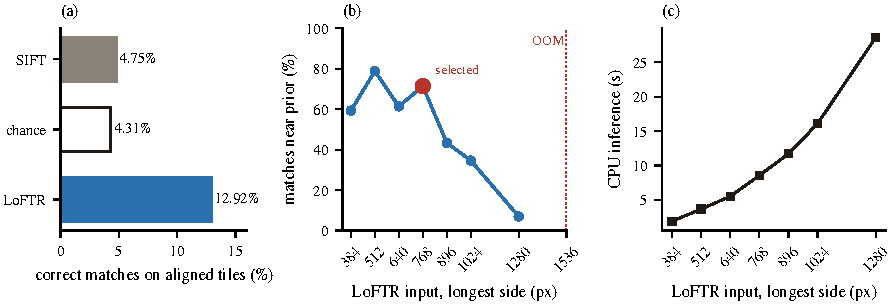
\includegraphics[width=\textwidth]{fig4_diagnostics}
\caption{Development diagnostics; no evaluation point was used. (a)~Share of correct matches on tiles already aligned by the printed corners, against the chance rate. (b)~Share of LoFTR matches within 1\,km of the printed-corner prior, by input size. The selection rule picked 768 pixels, and 1536 pixels ran out of memory on a 15\,GB machine. (c)~LoFTR inference time on the CPU.}
\label{fig:diag}
\end{figure*}

\begin{table}[t]
\centering
\caption{SIFT preprocessing variants. ``Near'': matches within 1\,km of the printed-corner prior. No variant produced a valid model.}
\label{tab:siftvar}
\footnotesize
\setlength{\tabcolsep}{2.6pt}
\begin{tabular}{lrrrrrc}
\toprule
Variant & KP scan & KP ref & Ratio & Near & Inl. & Valid \\
\midrule
\tabinput{tables/sift_variants.tex}
\bottomrule
\end{tabular}
\end{table}

\subsection{LoFTR is accurate but scale-sensitive}
At 768 pixels LoFTR produced 601 matches, of which MAGSAC++ kept 389 (64.7\%). The inlier reprojection RMSE is 6.4 working pixels (64\metre) in image space. That number measures how well the inliers fit the model, not positional accuracy. The resulting transform places the printed sheet corners a mean 199\metre{} from their graticule positions. Section~\ref{sec:datum} shows that most of this distance is a datum offset.

Table~\ref{tab:sweep} and Fig.~\ref{fig:diag}b show that the scale sensitivity is strong and not monotonic. The share of matches consistent with the prior is 59\% at 384 pixels, 79\% at 512, 61\% at 640, 71\% at 768 and only 7\% at 1280, the size we had originally planned to use. Had we kept 1280 pixels, LoFTR would have failed almost as completely as SIFT. In practice this sensitivity matters more than any small difference between matchers.

\begin{table}[t]
\centering
\caption{LoFTR input-size sweep (CPU). ``Res.'': effective ground resolution. ``Near'': matches within 1\,km of the printed-corner prior.}
\label{tab:sweep}
\footnotesize
\setlength{\tabcolsep}{3pt}
\begin{tabular}{rrrrrr}
\toprule
Side (px) & Res. (m) & Matches & Near & Near (\%) & Time (s) \\
\midrule
\tabinput{tables/sweep.tex}
\bottomrule
\end{tabular}
\end{table}

\subsection{Georeferenced output}
A homography cannot be stored as a GeoTIFF affine geotransform. We therefore resample the scan onto a north-up EPSG:32643 grid at 5\metre. Each output pixel is mapped back to the scan through the exact inverse chain (output pixel $\to$ metres $\to$ reference pixel $\to H^{-1}\to$ scan pixel), so bilinear interpolation is the only approximation. A unit test on a linear ramp confirms the mapping to within 0.02 grey levels.

We also tested the written files using only their own georeferencing. At 2{,}000 random points inside the neatline, the GeoTIFF sampled at the predicted coordinate returns the source scan pixel, with a mean absolute colour difference of 4.6. A deliberate 10\metre{} shift raises this to 14.8. Figure~\ref{fig:windows} draws OSM vectors on the LoFTR GeoTIFF. Railways, roads and the Cauvery fall on the 1926 linework to within a few tens of metres. That includes Mysore station, where neither method was fitted.

As an independent check we opened both GeoTIFFs in QGIS~3.44.14 LTR from a standalone PyQGIS script that uses none of our code. QGIS reads the same CRS, extent, size and 5\metre{} pixel size that the pipeline wrote. We loaded the raw OSM railways, rivers and major roads in WGS\,84 and let QGIS reproject them on the fly. Across the whole sheet they fall on the 1926 linework. Figure~\ref{fig:qgis} shows a 700\metre{} window around each held-out point. In every window the 1926 feature sits under LoFTR's predicted position, and is offset from the OSM truth by the reported error. At E11 the 1926 and OSM roads coincide, but the picked junction lies about 190\metre{} along the road from the OSM junction. This is what a mis-identified or moved junction would look like, and it supports our reading of E11 below.

\begin{figure*}[t]
\centering
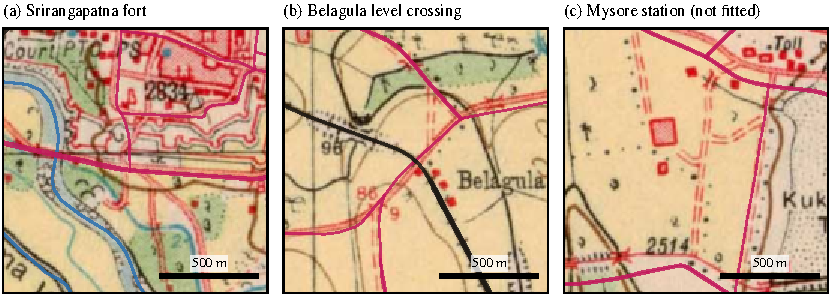
\includegraphics[width=\textwidth]{fig5_alignment_windows}
\caption{Windows of the LoFTR GeoTIFF with OSM vectors drawn using only the file's own geotransform. Black: railway. Blue: river. Magenta: major roads. (c)~lies about 4\,km from the nearest fitting point and contains no evaluation point.}
\label{fig:windows}
\end{figure*}

\begin{figure*}[t]
\centering
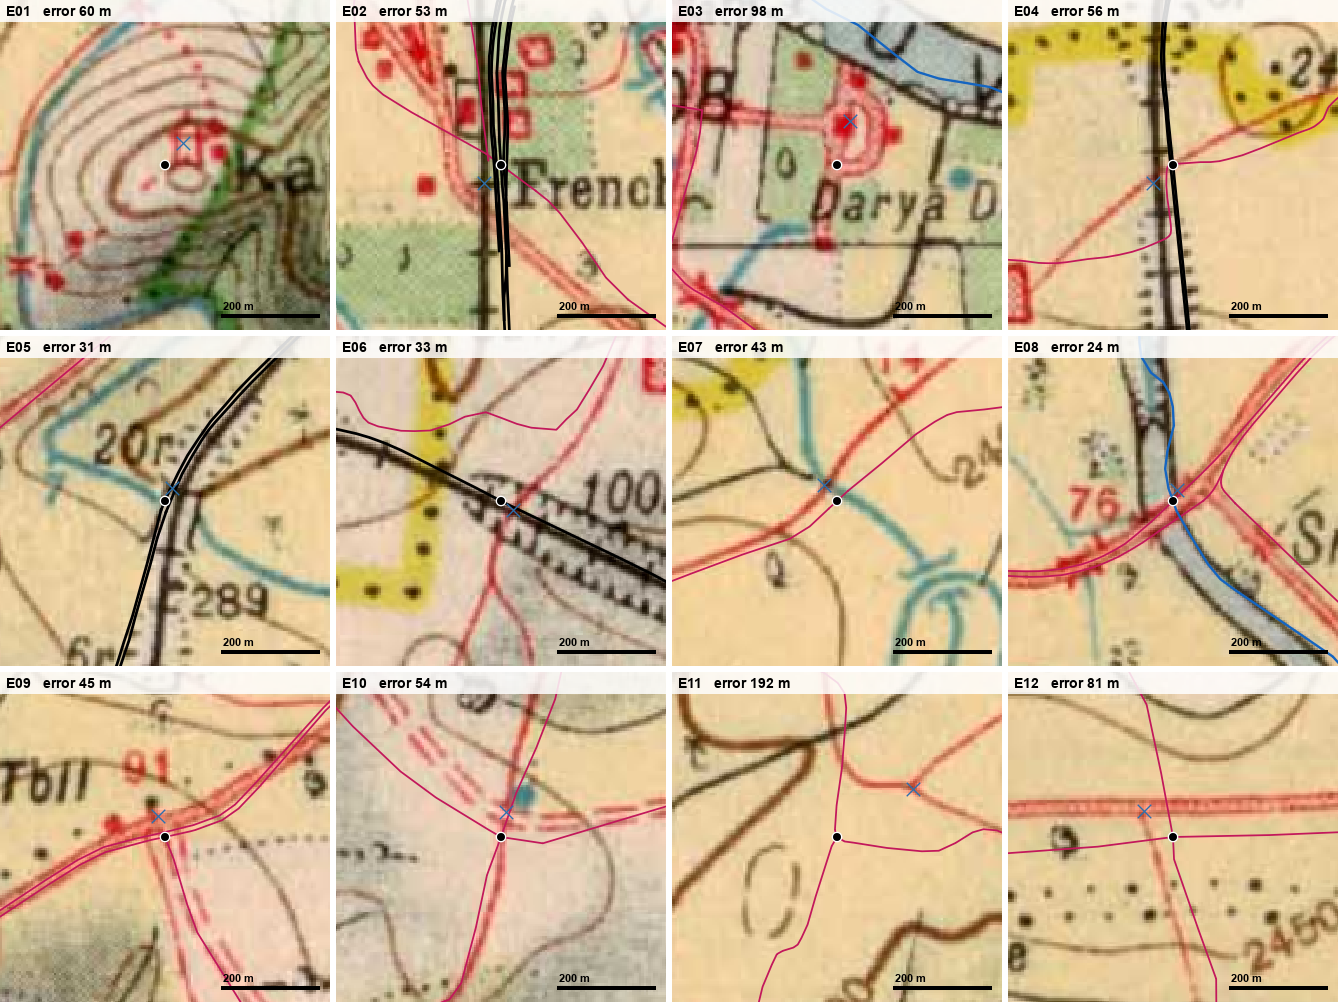
\includegraphics[width=0.92\textwidth]{fig12_qgis_points}
\caption{QGIS~3.44 render of the LoFTR GeoTIFF around each held-out point (700\metre{} windows, 200\metre{} scale bars). Magenta, black and blue lines: OSM roads, railways and rivers, reprojected by QGIS. Black dot: OSM truth. Blue cross: LoFTR's prediction. The distance between the two is the error in Table~\ref{tab:points}.}
\label{fig:qgis}
\end{figure*}

\subsection{Held-out accuracy}
Table~\ref{tab:results} gives the main result. LoFTR's median held-out error is 53.9\metre{} with an RMSE of 77.4\metre. The 7-point manual fit reaches 73.9\metre{} and 102.4\metre. At the 1:63,360 scale of the sheet, these RMSEs equal 1.22\,mm and 1.62\,mm on paper. Within 50\metre, LoFTR places 5 of 12 points and the manual fit 3. Within 100\metre, the counts are 11 and 9.

The 1947 US National Map Accuracy Standard~\citep{nmas1947} asks for 90\% of well-defined points within 1/50 inch at this scale, which is 32.2\metre. LoFTR meets it at 2 points and the manual fit at none. Neither result should be read as a statement about the original survey, because both include picking error, OSM error and a century of change.

Table~\ref{tab:points} and Fig.~\ref{fig:errors}a give the per-point errors. LoFTR is closer at 9 of 12 points. The median paired difference is $-31.7$\metre{} (Wilcoxon $W=13$, exact $p=0.043$), with a bootstrap 95\% interval of $[-44.0, +2.5]$\metre. Because the interval includes zero, we treat the advantage as suggestive but not established. Section~\ref{sec:robust} shows that this reading holds after accounting for spatial clustering and for the number of secondary tests.

The largest error belongs to E11, a low-confidence road junction in the north-west: 191.7\metre{} for LoFTR and 223.9\metre{} for the manual fit, in nearly the same direction. That pattern points to the point, not the methods: either a mis-identified junction or a realigned road. We kept E11 in all reported numbers. Without the three low-confidence points (E03, E11, E12), LoFTR's median and RMSE fall to 44.9\metre{} and 46.0\metre, and the manual fit's to 66.7\metre{} and 86.1\metre. This is a sensitivity check, not a replacement result.

\begin{table*}[t]
\centering
\caption{Held-out points. Truth is OSM geometry in EPSG:32643. $\Delta E,\Delta N$ are predicted minus true (m). Bold values are positional errors.}
\label{tab:points}
\small
\begin{tabular}{lllrrrrrrrr}
\toprule
& & & \multicolumn{2}{c}{Truth (m)} & \multicolumn{3}{c}{LoFTR} & \multicolumn{3}{c}{Manual} \\
\cmidrule(lr){4-5}\cmidrule(lr){6-8}\cmidrule(lr){9-11}
ID & Feature & Conf. & $E$ & $N$ & $\Delta E$ & $\Delta N$ & $e$ & $\Delta E$ & $\Delta N$ & $e$ \\
\midrule
\tabinput{tables/points.tex}
\bottomrule
\end{tabular}
\end{table*}

\begin{figure*}[t]
\centering
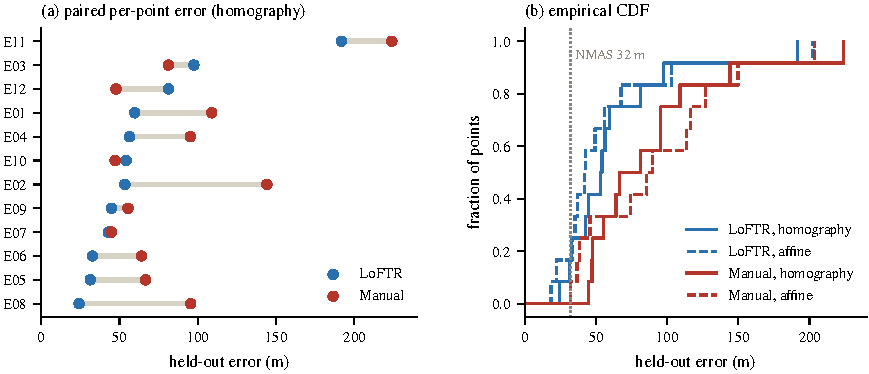
\includegraphics[width=\textwidth]{fig7_errors}
\caption{(a)~Per-point held-out error, sorted by LoFTR error. The grey bar spans the paired difference. (b)~Empirical CDF of the error for both methods and both transform models. The dotted line marks the NMAS threshold for this scale (32.2\metre).}
\label{fig:errors}
\end{figure*}

\subsection{Where the errors come from}
\paragraph{Bias.}
Both methods have a mean error vector clearly different from zero (Fig.~\ref{fig:components}). LoFTR's mean error is $(+9.7, +31.2)$\metre, and the bootstrap 95\% interval of its north component, $[5.6, 55.7]$\metre, excludes zero. The manual fit's mean error is $(+43.8, -34.9)$\metre, and both of its intervals exclude zero ($\Delta E\in[8.4, 84.7]$, $\Delta N\in[-65.6, -5.5]$). In the north-east, the manual errors at E01, E02, E04 and E08 all point south (Fig.~\ref{fig:vectors}b).

These four points lie near the edge of the manual fit's support. Only three of its seven fitting points are in the eastern third of the sheet, and only one, F09, is in the south. A homography fitted to seven unevenly spread points has two weakly constrained projective terms. This matches the gap between its fitting RMSE (55.6\metre) and its leave-one-out RMSE (146.9\metre) (Fig.~\ref{fig:methodc}).

\paragraph{Support.}
Error does not grow clearly with distance from support (Fig.~\ref{fig:distance}). For LoFTR, the Spearman correlation between a point's error and its distance to the nearest RANSAC inlier is $\rho=0.39$ ($p=0.21$; median distance 1.26\,km). For the manual fit, against the distance to the nearest fitting point, it is $\rho=-0.10$ ($p=0.75$; median 2.5\,km). Twelve points are too few to rule out a moderate effect, and the southern fifth of the sheet, where both methods extrapolate, has no evaluation points at all.

\begin{figure*}[t]
\centering
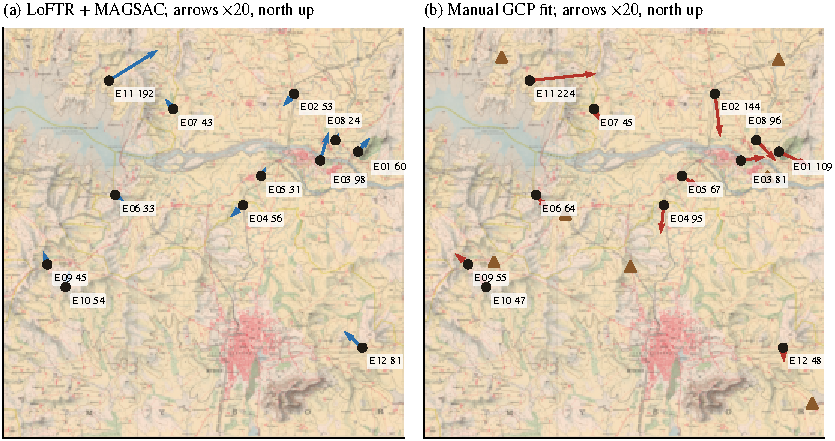
\includegraphics[width=\textwidth]{fig6_error_vectors}
\caption{Held-out error vectors ($\times20$, north up), labelled with the error in metres. Brown triangles in (b) are the seven fitting points used by the manual baseline.}
\label{fig:vectors}
\end{figure*}

\begin{figure}[t]
\centering
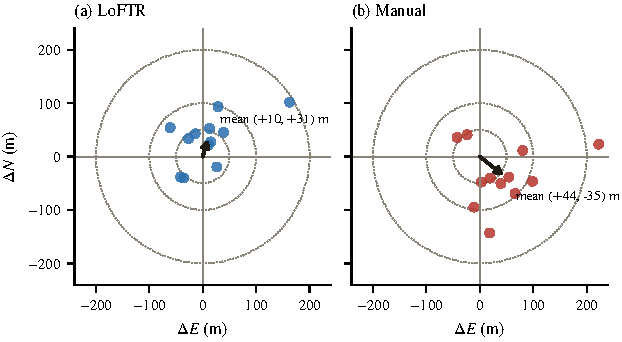
\includegraphics[width=\columnwidth]{fig8_error_components}
\caption{Error components (predicted minus true). Rings mark 50, 100 and 200\metre. Arrows show the mean bias.}
\label{fig:components}
\end{figure}

\begin{figure}[t]
\centering
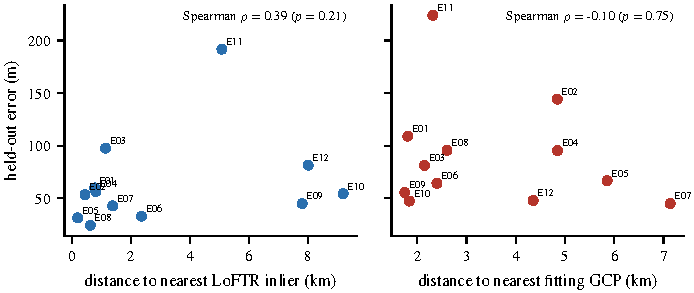
\includegraphics[width=\columnwidth]{fig10_distance}
\caption{Held-out error against distance to the nearest support: LoFTR inliers (left) and manual fitting points (right). Exploratory analysis.}
\label{fig:distance}
\end{figure}

\begin{figure}[t]
\centering
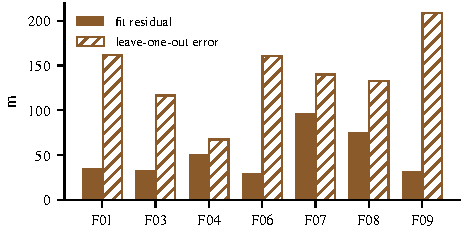
\includegraphics[width=\columnwidth]{fig11_methodc_fit}
\caption{Manual baseline: residual at each fitting point against the error when that point is left out of the fit.}
\label{fig:methodc}
\end{figure}

\subsection{Affine or projective?}
Re-estimating every model as an affine transform, with the same inputs, settings and seed, changes little. LoFTR goes from median 53.9 to 42.4\metre{} and RMSE 77.4 to 76.3\metre. The manual fit goes from median 73.9 to 87.8\metre{} and RMSE 102.4 to 105.5\metre. Under the affine model, LoFTR is closer at 10 of 12 points (Wilcoxon $p=0.016$, bootstrap interval $[-58.6, -5.1]$\metre). A flat, undistorted scan of a sheet this small has little perspective to model. The two extra degrees of freedom mostly add variance, most visibly in the sparsely constrained manual fit. We did not use this comparison to select anything.

\subsection{The datum of the printed graticule}
\label{sec:datum}
We measured the offset between true WGS\,84 positions and the positions implied by the printed graticule, read as if it were WGS\,84, at the seven fitting points (Fig.~\ref{fig:datum}). The median is $(-84, +53)$\metre, with robust spreads of 58\metre{} east and 95\metre{} north. LoFTR's correct development matches give a similar $(-128, +133)$\metre. PROJ's Kalianpur~1937 and~1975 parameters give $(-23$ to $-118, +159)$\metre{} at the sheet centre. All three estimates agree in direction. Together they support a datum shift of roughly 100--200\metre, which explains most of the 117--199\metre{} corner discrepancy reported above. The exact datum remains unidentified.

\begin{figure}[t]
\centering
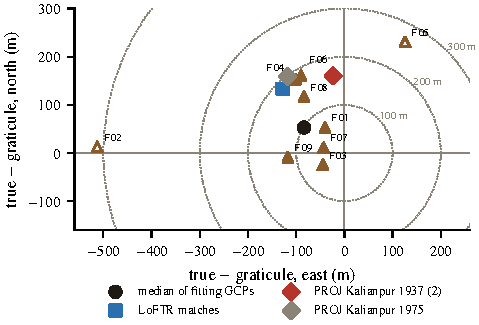
\includegraphics[width=\columnwidth]{fig9_datum}
\caption{True WGS\,84 position minus the position implied by the printed graticule at each fitting point. Hollow points were excluded by quality control. Larger markers are aggregate and PROJ estimates.}
\label{fig:datum}
\end{figure}

\subsection{Compute and reproducibility}
On the CPU, LoFTR took 18.3\,s end to end, 8.0\,s of it inference. SIFT took 14.6\,s and the manual fit 0.15\,s. Re-running LoFTR on an RTX~3050 Laptop GPU (4\,GB, CUDA~12.6, peak 1.06\,GB) with the frozen settings gave the same 601 matches and 389 inliers in 1.8\,s of inference. Floating-point differences between the devices move the transform by 1.9\metre{} on average and 8.5\metre{} at most across the sheet. The held-out RMSE becomes 77.2\metre{} against 77.4\metre. All reported numbers come from the CPU run. With warm caches, five repeated CPU runs took a median 6.5\,s for LoFTR (4.8\,s matching) and 7.2\,s for SIFT. The exact inputs are versioned in the repository, so a complete re-run reproduces every transform matrix, per-point error and summary statistic bit for bit on the original machine, in about five minutes. A continuous-integration job repeats the whole experiment on Linux (Ubuntu~24.04, the same pinned packages). There, every per-point error and summary statistic agrees to 0.01\metre; the transform matrices differ only in the last floating-point digits.

\section{Robustness and sensitivity}
\label{sec:robust}
All analyses in this section were added after the held-out evaluation. They test how far the conclusions depend on choices we made. None of them was used to change a parameter or a reported result. Table~\ref{tab:robust} summarises them and Fig.~\ref{fig:robust} shows three of them.

\begin{table}[t]
\centering
\caption{Post-hoc robustness checks. Distances in metres on the same 12 held-out points unless stated.}
\label{tab:robust}
\footnotesize
\setlength{\tabcolsep}{3pt}
\begin{tabularx}{\columnwidth}{>{\raggedright\arraybackslash}p{0.36\columnwidth}>{\raggedright\arraybackslash}X}
\toprule
Check & Result \\
\midrule
\tabinput{tables/robustness.tex}
\bottomrule
\end{tabularx}
\end{table}

\begin{figure*}[t]
\centering
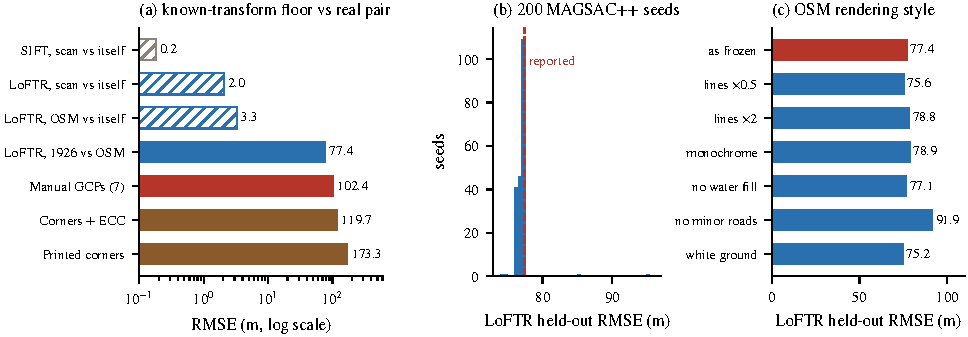
\includegraphics[width=\textwidth]{fig13_robustness}
\caption{(a)~RMSE on pairs with a known transform (hatched: the same image warped and matched against itself) compared with the real 1926--OSM pair and the classical baselines. (b)~LoFTR held-out RMSE over 200 explicitly seeded MAGSAC++ runs. (c)~LoFTR held-out RMSE for six alternative OSM renderings.}
\label{fig:robust}
\end{figure*}

\paragraph{Where the error comes from.}
To separate the matchers' own error from everything else, we warped each image by a known homography and matched it against itself. On the 1926 scan, LoFTR recovered the transform to 2.0\metre{} RMSE and SIFT to 0.2\metre; on the OSM render, the figures were 3.3\metre{} and 0.2\metre. Blur, noise and JPEG compression changed this by at most 0.4\metre. SIFT is therefore the more precise matcher whenever both images share a style. It fails on the real pair only because its descriptors do not carry across the gap between a 1926 lithograph and a vector rendering.

The other error sources are also small or measured:
\begin{itemize}
\item \emph{Projection.} Mapping a polyconic sheet (Everest spheroid, centred on the sheet) onto UTM~43N with one homography leaves at most 0.46\metre.
\item \emph{Scan geometry.} The printed neatline is straight to 0.4--1.4 pixels RMS (2--8\metre). Ground scale differs by 0.4\% between the two directions, which any affine or projective fit absorbs. The JPEG quality is about 79.
\item \emph{Colour plates.} The background tint meets the black neatline within one pixel on the west and east sides. Comparing north and south implies a tint-plate offset of 1.7 pixels (about 9\metre); the red, blue and brown line plates share no edge with the black plate and could not be measured.
\item \emph{Cartographic displacement.} Printed road bands are a median 35\metre{} wide on the ground (0.55\,mm on paper) and railways 10\metre. Where a road runs within 27.5\metre{} of a railway, one of them must be displaced by 12--25\metre; this happened at 28 of 550 sampled places.
\end{itemize}
With the matcher contributing only a few metres, the 50--100\metre{} held-out errors come mostly from the map itself, a century of change, OSM and our picking.

\paragraph{Stability of LoFTR.}
Over 200 explicitly seeded MAGSAC++ runs, LoFTR was always valid with 389--390 inliers. Its RMSE stayed between 76.2 and 77.4\metre{} in 90\% of runs, with a single outlier at 95.3\metre; SIFT was never valid. Six alternative OSM renderings, with thinner or thicker lines, no colour, no water fill, no minor roads or a white background, gave RMSEs of 75.2--91.9\metre{} and never failed. Removing minor roads was the most damaging change. Raising the match-confidence threshold to 0.3 would have lowered the median error to 37.5\metre, but higher thresholds raised it again, to 98.0\metre{} RMSE at 0.8; we kept the frozen choice of using every match.

\paragraph{Does LoFTR succeed by matching the truth features?}
The evaluation truth and LoFTR's reference both come from OSM. If LoFTR's accuracy came from matching the very features we score it on, removing those matches should hurt. For each test point we deleted every LoFTR match whose OSM location lay within 1, 2 or 3\,km, refitted and re-predicted that point. RMSE moved from 77.4 to 77.4, 78.4 and 80.6\metre, so the accuracy does not depend on local matches at the test points.

\paragraph{Statistics.}
Bootstrap intervals for the summary statistics are wide: LoFTR median 53.9\metre{} $[37.8, 70.6]$, manual 73.9\metre{} $[51.7, 102.3]$. Moran's $I$ found no spatial autocorrelation in the errors ($p=0.20$--$0.92$)~\citep{moran1950}. Grouping points into eight clusters joined within 3\,km and resampling clusters instead of points gave a median paired difference of $-31.7$\metre{} $[-44.0, -2.0]$; an exact sign-flip test over clusters gave $p=0.070$. Dropping the two landmark points, whose truth is a building or garden centroid rather than a crossing, gave $p=0.049$ with the same direction. We adjusted all 23 secondary tests, including those of Sections~\ref{sec:ext} and~\ref{sec:repick}, together with Holm's method~\citep{holm1979} and the Benjamini--Hochberg false-discovery rate~\citep{benjamini1995}. LoFTR versus georeferencing from the printed corners survives (Holm $p=0.012$), and so do the two comparisons against the manual fit refitted on the human re-pick (Holm $p=0.012$ and $0.032$; Section~\ref{sec:repick}). No comparison against the original manual fit does: the affine and landmark variants reach $q=0.07$--$0.14$. The primary comparison was the single test specified in advance; it stays at $p=0.043$, which we read as suggestive.

\paragraph{Classical baselines and the manual model.}
SIFT is a weak stand-in for classical map registration, so we added two standard classical baselines on the same points. Georeferencing from the four printed sheet corners alone reaches a median of 169.8\metre{} (RMSE 173.3\metre); most of that is the datum offset. Refining it by enhanced-correlation-coefficient (ECC) alignment~\citep{evangelidis2008} of the colour-separated linework brings it to 99.5\metre{} (RMSE 119.7\metre). LoFTR was closer than corners-plus-ECC at 9 of 12 points ($p=0.021$, Holm $p=0.38$). The manual baseline had received no tuning, so we let it choose its transform model by leave-one-out error on its own seven fitting points. It chose a similarity transform (median 90.2\metre, RMSE 106.2\metre), slightly worse on the held-out points than the frozen homography.

\paragraph{Development thresholds.}
The input-size rule picks 768 pixels at every prior radius from 0.5 to 2\,km; ranking by the fraction instead of the count of near matches would pick 512. LoFTR's share of correct matches on aligned tiles exceeds chance at every radius from 200 to 1000\metre{} (1.7--14 times chance). SIFT stays within 1.0--1.5 times chance and is marginally above it only at 300\metre{} (uncorrected $p=0.04$).

\paragraph{Datum.}
The seven fitting points place the printed graticule $(-84, +53)$\metre{} from WGS\,84, with bootstrap intervals of $[-101, -43]$ east and $[-9, +153]$ north. The 12 evaluation points, an independent sample used here without any method, give $(-105, +105)$\metre, with $[-145, -74]$ and $[+81, +138]$. Together they indicate an offset of roughly 100--150\metre{}, with the true position lying north-west of where the printed graticule places it.

\section{Other matchers and other transform models}
\label{sec:ext}
Two questions are left open by the main comparison: is LoFTR special, or would any modern learned matcher do; and does the single homography limit accuracy? We answered both after the evaluation, under the same rules as the original methods. Settings were chosen on development data only, by criteria written down first, and then scored once on the 12 locked points. Table~\ref{tab:ext} and Fig.~\ref{fig:ext} give the results.

\begin{table}[t]
\centering
\caption{Post-hoc method extensions. Distances in metres on the 12 held-out points.}
\label{tab:ext}
\footnotesize
\setlength{\tabcolsep}{3pt}
\begin{tabularx}{\columnwidth}{>{\raggedright\arraybackslash}p{0.33\columnwidth}>{\raggedright\arraybackslash}X}
\toprule
Extension & Result \\
\midrule
\tabinput{tables/extensions.tex}
\bottomrule
\end{tabularx}
\end{table}

\begin{figure*}[t]
\centering
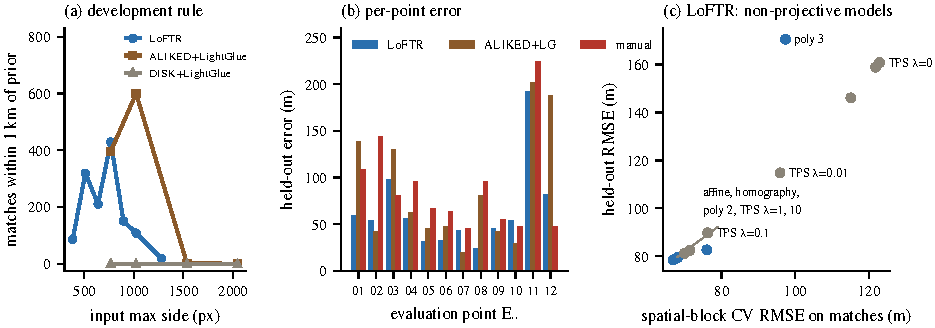
\includegraphics[width=\textwidth]{fig14_extensions}
\caption{(a)~Matches within 1\,km of the printed-corner prior against input size, the development rule used to choose the input size of every learned matcher. (b)~Held-out error per point for LoFTR, ALIKED with LightGlue and the manual fit. (c)~Non-projective models fitted to LoFTR's 390 inlier matches: cross-validation error on the matches against held-out RMSE.}
\label{fig:ext}
\end{figure*}

\paragraph{Sparse learned matchers.}
We paired LightGlue~\citep{lindenberger2023lightglue} with two learned keypoint detectors, DISK~\citep{tyszkiewicz2020disk} and ALIKED~\citep{zhao2023aliked}, using the Kornia implementations and pretrained weights (4096 keypoints per image, LightGlue's default filter). Matches went into the frozen MAGSAC++ estimator with the 3-pixel threshold at the matcher's resolution. As for LoFTR, the input size was the one with the most matches within 1\,km of the printed-corner prior.

DISK with LightGlue returned 0--2 matches at every input size from 768 to 2048 pixels, so it produced no transform and fails like SIFT. Its features are not useless: on the prior-aligned tiles of Fig.~\ref{fig:diag}a, 53\% of its matches were correct against 4.3\% by chance, far better than SIFT (4.75\%) and even LoFTR (12.9\%); ALIKED reached 27\%. It fails at finding the global correspondence, not at matching the linework locally. ALIKED with LightGlue worked at 768 and 1024 pixels and collapsed above that, the same scale sensitivity LoFTR shows (Fig.~\ref{fig:ext}a). At the selected 1024 pixels it gave 216 inliers out of 604 matches and a held-out median of 54.6\metre, almost LoFTR's, but an RMSE of 104.9\metre, driven by E01, E03 and E12. LoFTR was closer at 8 of 12 points ($p=0.15$). So LoFTR is not the only learned matcher that crosses the style gap, but it was the more reliable of the two that did.

\paragraph{Non-projective models.}
We replaced the homography by second- and third-order polynomials and by thin-plate splines~\citep{bookstein1989tps} with seven smoothing values. For LoFTR they were fitted to its 390 MAGSAC++ inlier matches, and the model was chosen by $4\times4$ spatial-block cross-validation on those matches. For the manual baseline they were fitted to its seven points and chosen by leave-one-out. Both rules picked the affine model. Its held-out RMSE was 78.5\metre{} from LoFTR's matches against 79.4\metre{} for a least-squares homography on the same matches (12 points, $p=0.85$), and 105.5\metre{} from the manual points. Flexible models did worse in cross-validation and on the held-out points: a cubic polynomial reached 170.6\metre{} and an unsmoothed spline 160.8\metre. Smoothed splines approached the affine result as the smoothing grew. One caveat applies: the inliers were selected by a homography with a tolerance of about 135\metre, so a local model can only redistribute residuals within that band. Even so, the cross-validation shows no smooth distortion that the matches can resolve better than a global model. On this sheet the limit is the content and its change, not the transform family.

\section{A blind human re-pick}
\label{sec:repick}
The original control points were proposed with AI assistance and reviewed by the author after the held-out results existed. To test how much the manual baseline and the evaluation depend on them, the author re-picked every point blind and timed, after all other analyses were complete. A local picking tool (\texttt{mapalign.pickweb}) showed a window of the scan centred on the printed-corner estimate, never on an earlier pick, next to the OSM render with the target marked. It recorded the click in full-resolution pixels, the seconds from display to acceptance and a confidence flag. Three kits were picked: the 12 evaluation points (truth unchanged, only the historical pixel replaced), the 9 fitting points (Method~C refitted with the frozen QC rule), and 57 new candidates in the 15 design cells that had no evaluation point, including the south and Mysore city. Table~\ref{tab:repick} gives the results.

\begin{table}[t]
\centering
\caption{Blind, timed human re-pick. Distances in metres, as median / RMSE on the held-out points; $p$ from the exact Wilcoxon test, unadjusted (adjusted values in Section~\ref{sec:robust}).}
\label{tab:repick}
\footnotesize
\setlength{\tabcolsep}{3pt}
\begin{tabularx}{\columnwidth}{>{\raggedright\arraybackslash}p{0.33\columnwidth}>{\raggedright\arraybackslash}X}
\toprule
Re-pick & Result \\
\midrule
\tabinput{tables/repick.tex}
\bottomrule
\end{tabularx}
\end{table}

\paragraph{Evaluation pixels.}
The two pickers agreed closely: the median gap was 7.3 pixels (about 39\metre), and 10 of 12 points agreed within 20 pixels. The exceptions were E04 (58 pixels) and E12 (76 pixels), where the re-pick lies further along the same road. Re-scored on the new pixels, the frozen transforms keep their order: LoFTR has a median of 50.8\metre{} and the manual fit 106.9\metre, and LoFTR is closer at 9 of 12 points ($p=0.027$). LoFTR's RMSE rises to 146.2\metre, almost entirely from E12. The pick-to-pick spread is larger than the $\pm27$\metre{} assumed in Section~\ref{sec:gcp}, so picking is a larger share of the error budget than we had allowed for.

\paragraph{Fitting points.}
The frozen QC rule removed only F02 this time (F05 was re-picked 49 pixels from its original position and passed), so the refitted manual baseline used eight points. On the original evaluation pixels it reached a median of 123.7\metre{} and an RMSE of 151.2\metre, against 73.9 and 102.4\metre{} for the original fit. LoFTR was closer at all 12 points ($p=0.0005$, Holm $p=0.012$). With both the fitting and the evaluation pixels from the human re-pick, the manual fit reached 142.4\metre{} (RMSE 208.9\metre) and LoFTR was closer at 11 of 12 points ($p=0.0015$, Holm $p=0.032$). A homography from a handful of points is therefore sensitive to which points pass quality control and to small differences in where they are clicked. The re-pick took 150\,s for the nine fitting points and 121\,s for the twelve evaluation points, a median of 9--12\,s per point, against 18\,s of computation for LoFTR on a CPU.

\paragraph{Supplementary points.}
None of the 57 candidates was skipped, and 39 were marked confident. Both methods had a median error of about 230\metre{} on them (RMSE 422 and 419\metre), with no difference between them ($p=0.38$). These errors do not measure georeferencing. The two transforms never disagree by more than 155\metre{} anywhere on the points, yet at 21 points both are more than 300\metre{} off, and at five more than 800\metre. At those points the picked 1926 feature is not the OSM feature: a nearby look-alike was picked, or the feature postdates the sheet. On the 39 confident points the medians were 122.4\metre{} for LoFTR and 165.6\metre{} for the manual fit (LoFTR closer at 22, $p=0.13$). The pick file is hashed and kept, but we do not use these points as evidence about accuracy in the south. They show instead that deciding whether a feature existed in 1926 is the hard part of building a held-out set, and that a picker with no instruction to skip will mostly not skip.

\section{Discussion}
Three findings stand out on this sheet. First, a matcher pretrained on outdoor photographs transfers to a hand-drawn 1926 lithograph against a vector rendering well enough to produce a usable alignment, while SIFT does not transfer at all. The aligned-tile test (Fig.~\ref{fig:diag}a) shows that SIFT's failure is in the descriptors, not in the robust estimation. On pairs that share a style, SIFT is in fact the more precise matcher (Section~\ref{sec:robust}). LoFTR is not unique in this: ALIKED with LightGlue also produced a usable alignment, though a less reliable one, while DISK with LightGlue did not (Section~\ref{sec:ext}). Second, LoFTR's success depends on the input scale, and not monotonically, and ALIKED behaved the same way. The scale was chosen by a rule fixed in advance, but a different rule could have produced failure, and practitioners should expect to sweep it. Third, the manual baseline's weakness here is coverage and fragility, not precision. With seven or eight usable points it extrapolates over much of the sheet, and a blind re-pick of the same features by the same person moved its median error from 74 to 124\metre{} (Section~\ref{sec:repick}).

The absolute numbers should be read against the sources of error that no method can remove. The matchers themselves contribute only a few metres. OSM geometry is plausibly accurate to 5--20\metre, and two pickers clicking the same feature differ by a median of about 39\metre. Cartographic generalisation displaces some features by 12--25\metre, and many features have shifted since 1926. A median of 54\metre{} is about 0.85\,mm on the printed sheet: close to the drafting limit of a one-inch map, and well above the NMAS threshold.

\paragraph{Limitations.}
\begin{itemize}
\item The study uses one sheet and one rendering style, so it does not support general claims about historical maps.
\item Only 12 evaluation points were available, none in the southern fifth of the sheet or in Mysore city. The 57 supplementary points picked later are dominated by identification errors (Section~\ref{sec:repick}), so results there remain untested.
\item The quality-control rule kept only points consistent with a smooth offset from the printed grid. Points in locally distorted areas were therefore excluded, which probably makes every method's absolute error look better than a random sample would.
\item All candidate points were OSM road, rail and water crossings or landmarks, the same kind of linework LoFTR matches; other feature types are untested.
\item The original control points were proposed with AI assistance and accepted by the author after the held-out results existed. The author's blind re-pick is a second picker, not an independent expert; the truth coordinates of the evaluation points still come from the original selection, and the manual baseline is not a measure of expert human georeferencing.
\item Classical registration is represented by SIFT, printed corners and ECC, not by a dedicated road-network matcher.
\item Three development settings were changed after initial failures, although all were frozen before the evaluation data existed.
\item The two sparse learned matchers and the non-projective models were added after the evaluation; they followed the same selection rules but were not part of the frozen plan. Other detector-free matchers and LoFTR inputs above 1280 pixels were not tested; at 1536 pixels LoFTR ran out of memory.
\end{itemize}

\section{Conclusion}
On sheet 57\,D/11 of 1926, LoFTR with MAGSAC++ georeferenced the scan to a held-out median error of 54\metre{} and an RMSE of 77\metre. A 7-point manual fit reached 74\metre{} and 102\metre. SIFT failed, at or barely above chance level even on pre-aligned tiles, although it is highly precise on same-style pairs. The comparison favours LoFTR over the original manual fit, but with 12 points and after correcting for secondary tests it is not decisive. Against a manual fit rebuilt from a blind, timed human re-pick, LoFTR was closer at every point, and that difference survives the correction. LoFTR clearly outperforms georeferencing from the printed corners alone. The matchers contribute only a few metres of error; most of it comes from the map and a century of change. Affine and projective models performed alike, and more flexible models did not help. ALIKED with LightGlue also works, with a similar median but a heavier tail; DISK with LightGlue does not. The printed graticule sits roughly 100\metre{} from WGS\,84.

The most useful next steps are a re-pick by an independent expert, held-out points in the south and in Mysore city chosen with an explicit rule for skipping features that may postdate the sheet, and the same protocol applied to more sheets and to several editions of the same sheet. The repository includes the kits and the picking tools for the first two; for the third, edition-to-edition alignment should be much easier than alignment to OSM and would separate map error from change. Code, provenance records and every intermediate output are available in the repository.

\paragraph{Data and code availability.}
The repository contains the pipeline, the configuration as frozen, both GCP files with their selection protocol, all metrics and per-point errors, all robustness analyses (\texttt{mapalign.robustness} and \texttt{mapalign.robustness\_extra}), the method extensions (\texttt{mapalign.extensions}), the blind re-pick kits, the human re-pick files and two timed picking tools (\texttt{mapalign.picktool} and the browser-based \texttt{mapalign.pickweb}), a log of every design decision (\texttt{docs/DECISIONS.md}), and the script that regenerates every figure and table in this paper (\texttt{paper/make\_figures.py}). The exact inputs (scan and OSM extracts) are versioned with their checksums. The LoFTR weights are verified by SHA-256 and mirrored as a release asset. A continuous-integration workflow re-runs the experiment on Linux and compares it with the committed results.

\paragraph{Acknowledgements.}
Map scan: the Old Survey of India Maps collection compiled by John Brown (Zenodo, CC\,BY\,4.0). Modern data \textcopyright{} OpenStreetMap contributors, ODbL.

\small
\bibliographystyle{unsrtnat}
\bibliography{refs}

\end{document}
